% Architecture concept: control plane and data plane
% include with % Architecture concept: control plane and data plane
% include with % Architecture concept: control plane and data plane
% include with % Architecture concept: control plane and data plane
% include with \input{chapters/architecture}
% Needs only TikZ + the positioning library (already loaded via forest in main.tex)
\begin{figure}[htbp]
  \centering
  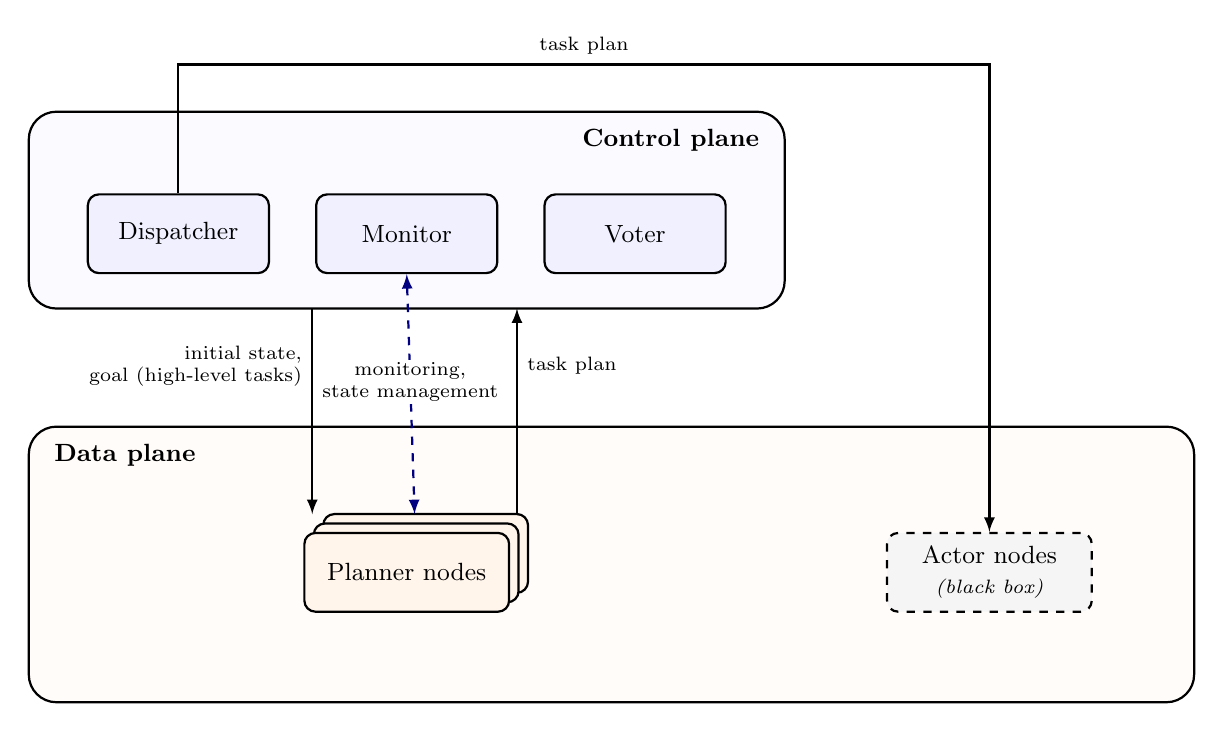
\begin{tikzpicture}[
      >=latex,
      font=\small,
      plane/.style={draw, thick, rounded corners=10pt},
      ctrl/.style ={draw, thick, rounded corners=4pt, fill=blue!6, align=center,
                    minimum width=2.3cm, minimum height=1.0cm},
      data/.style ={draw, thick, rounded corners=4pt, fill=orange!8, align=center,
                    minimum width=2.6cm, minimum height=1.0cm},
      planelbl/.style={font=\small\bfseries, anchor=north west},
      flow/.style ={->, thick},
    ]
    % ---------------- Control plane ----------------
    \draw[plane, fill=blue!2] (0,0) rectangle (9.6,2.5);
    \node[planelbl, anchor=north east] at (9.4,2.4) {Control plane};
    \node[ctrl] (disp) at (1.9,0.95) {Dispatcher};
    \node[ctrl] (mon)  at (4.8,0.95) {Monitor};
    \node[ctrl] (vot)  at (7.7,0.95) {Voter};

    % ---------------- Data plane ----------------
    \draw[plane, fill=orange!2] (0,-5.0) rectangle (14.8,-1.5);
    \node[planelbl] at (0.2,-1.6) {Data plane};

    % Planner nodes (stack = replicated nodes)
    \foreach \d in {0.24,0.12} {
      \node[data] at (4.8+\d,-3.35+\d) {};
    }
    \node[data] (plan) at (4.8,-3.35) {Planner nodes};

    % Actor nodes: single black-box component (not replicated)
    \node[data, dashed, fill=black!4] (act) at (12.2,-3.35) {Actor nodes\\{\scriptsize\itshape (black box)}};

    % ---------------- Interactions ----------------
    % Control plane <-> planner nodes (top of the node stack at y = -2.61)
    \draw[flow] (3.6,0) -- node[left, align=right, font=\scriptsize, pos=0.28]
      {initial state,\\goal (high-level tasks)} (3.6,-2.61);
    \draw[flow] (6.2,-2.61) -- node[right, font=\scriptsize, pos=0.72] {task plan} (6.2,0);

    % Monitor <-> planner nodes: monitoring and state management
    \draw[<->, thick, dashed, blue!50!black] (mon.south) -- node[fill=white, align=center,
      font=\scriptsize, pos=0.45, inner sep=1pt, text=black] {monitoring,\\state management} (4.9,-2.61);

    % Dispatcher -> actor nodes
    \draw[flow] (disp.north) |- node[above, pos=0.75, font=\scriptsize] {task plan}
      (12.2,3.1) -- (act.north);
  \end{tikzpicture}

  \caption[Architecture concept with control and data plane]{%
    Initial architecture concept with control plane and data plane.}
  \label{fig:architecture}
\end{figure}

% Needs only TikZ + the positioning library (already loaded via forest in main.tex)
\begin{figure}[htbp]
  \centering
  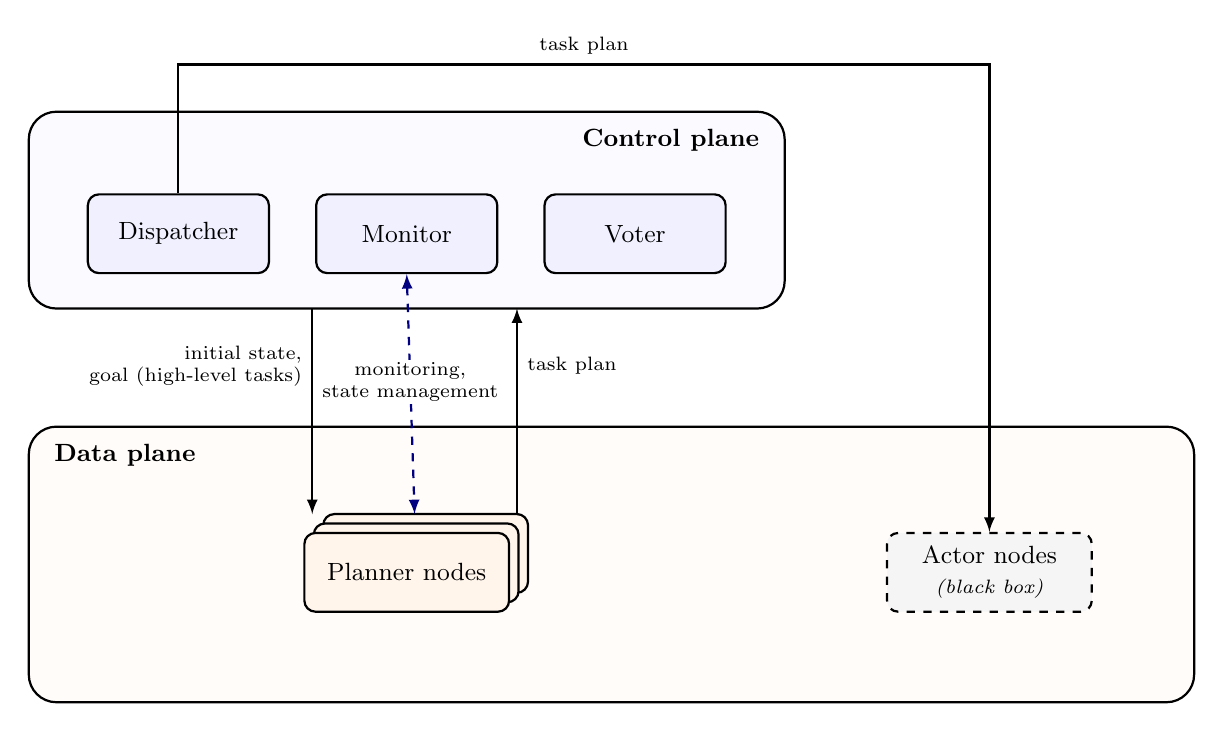
\begin{tikzpicture}[
      >=latex,
      font=\small,
      plane/.style={draw, thick, rounded corners=10pt},
      ctrl/.style ={draw, thick, rounded corners=4pt, fill=blue!6, align=center,
                    minimum width=2.3cm, minimum height=1.0cm},
      data/.style ={draw, thick, rounded corners=4pt, fill=orange!8, align=center,
                    minimum width=2.6cm, minimum height=1.0cm},
      planelbl/.style={font=\small\bfseries, anchor=north west},
      flow/.style ={->, thick},
    ]
    % ---------------- Control plane ----------------
    \draw[plane, fill=blue!2] (0,0) rectangle (9.6,2.5);
    \node[planelbl, anchor=north east] at (9.4,2.4) {Control plane};
    \node[ctrl] (disp) at (1.9,0.95) {Dispatcher};
    \node[ctrl] (mon)  at (4.8,0.95) {Monitor};
    \node[ctrl] (vot)  at (7.7,0.95) {Voter};

    % ---------------- Data plane ----------------
    \draw[plane, fill=orange!2] (0,-5.0) rectangle (14.8,-1.5);
    \node[planelbl] at (0.2,-1.6) {Data plane};

    % Planner nodes (stack = replicated nodes)
    \foreach \d in {0.24,0.12} {
      \node[data] at (4.8+\d,-3.35+\d) {};
    }
    \node[data] (plan) at (4.8,-3.35) {Planner nodes};

    % Actor nodes: single black-box component (not replicated)
    \node[data, dashed, fill=black!4] (act) at (12.2,-3.35) {Actor nodes\\{\scriptsize\itshape (black box)}};

    % ---------------- Interactions ----------------
    % Control plane <-> planner nodes (top of the node stack at y = -2.61)
    \draw[flow] (3.6,0) -- node[left, align=right, font=\scriptsize, pos=0.28]
      {initial state,\\goal (high-level tasks)} (3.6,-2.61);
    \draw[flow] (6.2,-2.61) -- node[right, font=\scriptsize, pos=0.72] {task plan} (6.2,0);

    % Monitor <-> planner nodes: monitoring and state management
    \draw[<->, thick, dashed, blue!50!black] (mon.south) -- node[fill=white, align=center,
      font=\scriptsize, pos=0.45, inner sep=1pt, text=black] {monitoring,\\state management} (4.9,-2.61);

    % Dispatcher -> actor nodes
    \draw[flow] (disp.north) |- node[above, pos=0.75, font=\scriptsize] {task plan}
      (12.2,3.1) -- (act.north);
  \end{tikzpicture}

  \caption[Architecture concept with control and data plane]{%
    Initial architecture concept with control plane and data plane.}
  \label{fig:architecture}
\end{figure}

% Needs only TikZ + the positioning library (already loaded via forest in main.tex)
\begin{figure}[htbp]
  \centering
  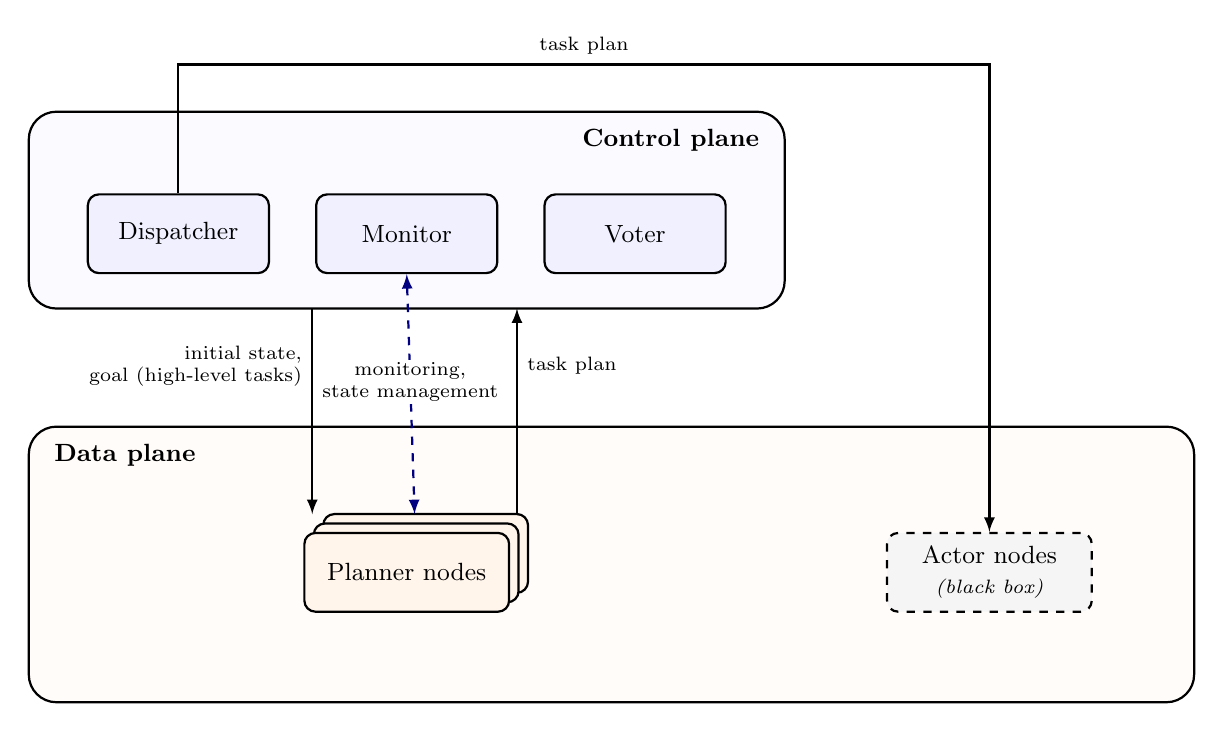
\begin{tikzpicture}[
      >=latex,
      font=\small,
      plane/.style={draw, thick, rounded corners=10pt},
      ctrl/.style ={draw, thick, rounded corners=4pt, fill=blue!6, align=center,
                    minimum width=2.3cm, minimum height=1.0cm},
      data/.style ={draw, thick, rounded corners=4pt, fill=orange!8, align=center,
                    minimum width=2.6cm, minimum height=1.0cm},
      planelbl/.style={font=\small\bfseries, anchor=north west},
      flow/.style ={->, thick},
    ]
    % ---------------- Control plane ----------------
    \draw[plane, fill=blue!2] (0,0) rectangle (9.6,2.5);
    \node[planelbl, anchor=north east] at (9.4,2.4) {Control plane};
    \node[ctrl] (disp) at (1.9,0.95) {Dispatcher};
    \node[ctrl] (mon)  at (4.8,0.95) {Monitor};
    \node[ctrl] (vot)  at (7.7,0.95) {Voter};

    % ---------------- Data plane ----------------
    \draw[plane, fill=orange!2] (0,-5.0) rectangle (14.8,-1.5);
    \node[planelbl] at (0.2,-1.6) {Data plane};

    % Planner nodes (stack = replicated nodes)
    \foreach \d in {0.24,0.12} {
      \node[data] at (4.8+\d,-3.35+\d) {};
    }
    \node[data] (plan) at (4.8,-3.35) {Planner nodes};

    % Actor nodes: single black-box component (not replicated)
    \node[data, dashed, fill=black!4] (act) at (12.2,-3.35) {Actor nodes\\{\scriptsize\itshape (black box)}};

    % ---------------- Interactions ----------------
    % Control plane <-> planner nodes (top of the node stack at y = -2.61)
    \draw[flow] (3.6,0) -- node[left, align=right, font=\scriptsize, pos=0.28]
      {initial state,\\goal (high-level tasks)} (3.6,-2.61);
    \draw[flow] (6.2,-2.61) -- node[right, font=\scriptsize, pos=0.72] {task plan} (6.2,0);

    % Monitor <-> planner nodes: monitoring and state management
    \draw[<->, thick, dashed, blue!50!black] (mon.south) -- node[fill=white, align=center,
      font=\scriptsize, pos=0.45, inner sep=1pt, text=black] {monitoring,\\state management} (4.9,-2.61);

    % Dispatcher -> actor nodes
    \draw[flow] (disp.north) |- node[above, pos=0.75, font=\scriptsize] {task plan}
      (12.2,3.1) -- (act.north);
  \end{tikzpicture}

  \caption[Architecture concept with control and data plane]{%
    Initial architecture concept with control plane and data plane.}
  \label{fig:architecture}
\end{figure}

% Needs only TikZ + the positioning library (already loaded via forest in main.tex)
\begin{figure}[H]
  \centering
  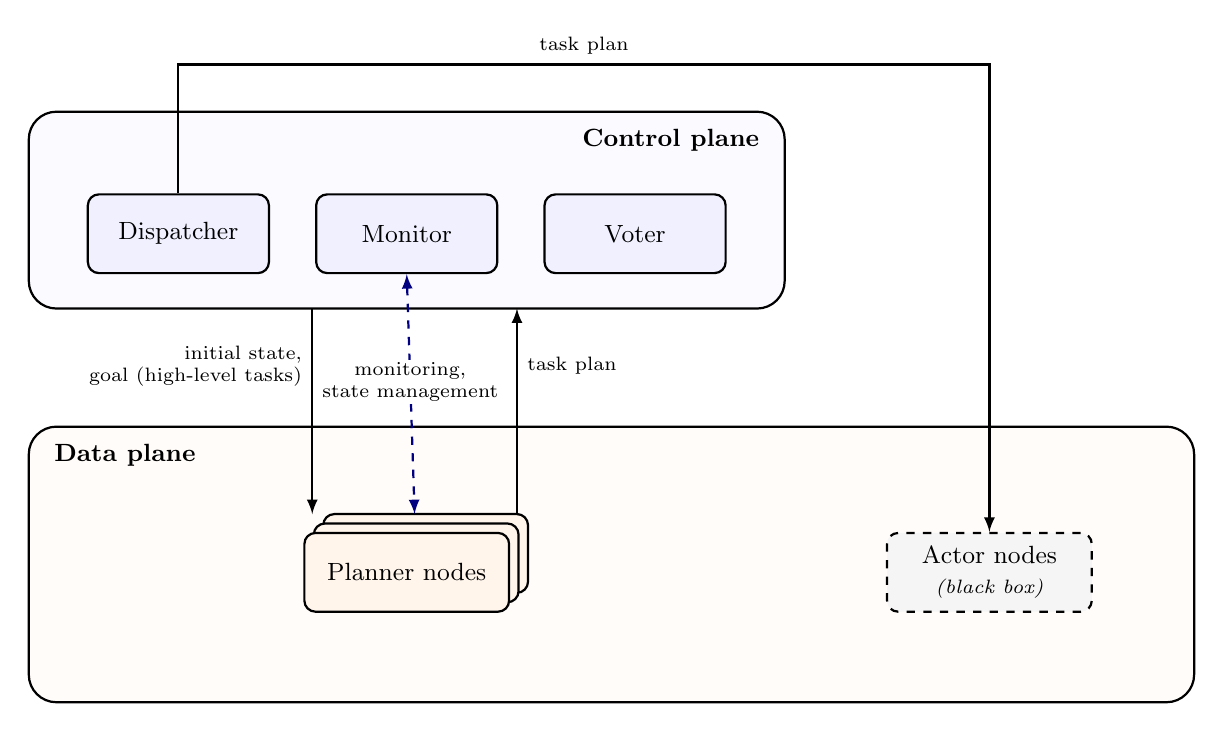
\begin{tikzpicture}[
      >=latex,
      font=\small,
      plane/.style={draw, thick, rounded corners=10pt},
      ctrl/.style ={draw, thick, rounded corners=4pt, fill=blue!6, align=center,
                    minimum width=2.3cm, minimum height=1.0cm},
      data/.style ={draw, thick, rounded corners=4pt, fill=orange!8, align=center,
                    minimum width=2.6cm, minimum height=1.0cm},
      planelbl/.style={font=\small\bfseries, anchor=north west},
      flow/.style ={->, thick},
    ]
    % ---------------- Control plane ----------------
    \draw[plane, fill=blue!2] (0,0) rectangle (9.6,2.5);
    \node[planelbl, anchor=north east] at (9.4,2.4) {Control plane};
    \node[ctrl] (disp) at (1.9,0.95) {Dispatcher};
    \node[ctrl] (mon)  at (4.8,0.95) {Monitor};
    \node[ctrl] (vot)  at (7.7,0.95) {Voter};

    % ---------------- Data plane ----------------
    \draw[plane, fill=orange!2] (0,-5.0) rectangle (14.8,-1.5);
    \node[planelbl] at (0.2,-1.6) {Data plane};

    % Planner nodes (stack = replicated nodes)
    \foreach \d in {0.24,0.12} {
      \node[data] at (4.8+\d,-3.35+\d) {};
    }
    \node[data] (plan) at (4.8,-3.35) {Planner nodes};

    % Actor nodes: single black-box component (not replicated)
    \node[data, dashed, fill=black!4] (act) at (12.2,-3.35) {Actor nodes\\{\scriptsize\itshape (black box)}};

    % ---------------- Interactions ----------------
    % Control plane <-> planner nodes (top of the node stack at y = -2.61)
    \draw[flow] (3.6,0) -- node[left, align=right, font=\scriptsize, pos=0.28]
      {initial state,\\goal (high-level tasks)} (3.6,-2.61);
    \draw[flow] (6.2,-2.61) -- node[right, font=\scriptsize, pos=0.72] {task plan} (6.2,0);

    % Monitor <-> planner nodes: monitoring and state management
    \draw[<->, thick, dashed, blue!50!black] (mon.south) -- node[fill=white, align=center,
      font=\scriptsize, pos=0.45, inner sep=1pt, text=black] {monitoring,\\state management} (4.9,-2.61);

    % Dispatcher -> actor nodes
    \draw[flow] (disp.north) |- node[above, pos=0.75, font=\scriptsize] {task plan}
      (12.2,3.1) -- (act.north);
  \end{tikzpicture}

  \caption[Architecture concept with control and data plane]{%
    Initial architecture concept with control plane and data plane.}
  \label{fig:architecture}
\end{figure}
